\documentclass{beamer}

\usepackage{tikz}
\usetikzlibrary{arrows,positioning}

\title{Solving Traffic Flow Problems with Linear Algebra}

\date{\today}

\begin{document}

\begin{frame}
    \titlepage
\end{frame}

\section{Introduction}

\begin{frame}{Traffic Flow Problems}
    Analyze the flow of traffic through a network of roads.
    \begin{itemize}
        \item \textbf{Nodes} represent intersections.
        \item \textbf{Edges} represent roads connecting intersections.
        \item \textbf{Flow variables} assigned to each road segment.
    \end{itemize}
\end{frame}

\section{Setting Up the Equations}

\begin{frame}{Example Traffic Network}
    \begin{figure}
        \centering
        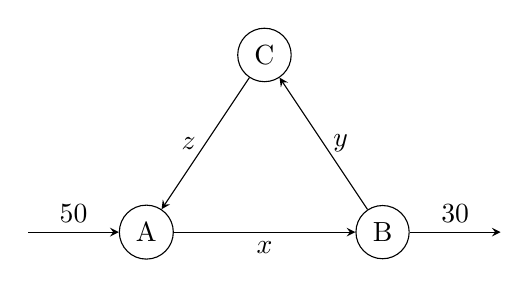
\begin{tikzpicture}[scale=1.5,>=stealth]
            % Nodes
            \node[circle,draw] (A) at (0,0) {A};
            \node[circle,draw] (B) at (2,0) {B};
            \node[circle,draw] (C) at (1,1.5) {C};
            % Edges
            \draw[->] (A) -- node[below]{$x$} (B);
            \draw[->] (B) -- node[right]{$y$} (C);
            \draw[->] (C) -- node[left]{$z$} (A);
            % External flows
            \draw[->] (-1,0) -- node[above]{$50$} (A);
            \draw[->] (B) -- node[above]{$30$} (3,0);
        \end{tikzpicture}
        \caption{Traffic Network Diagram}
    \end{figure}
\end{frame}

\begin{frame}{Writing the Equations}
    Based on the conservation of flow at each node:
    \begin{itemize}
        \item \textbf{Node A}:
        \[
        50 + z = x
        \]
        \item \textbf{Node B}:
        \[
        x = y + 30
        \]
        \item \textbf{Node C}:
        \[
        y = z
        \]
    \end{itemize}
\end{frame}

\section{Solving the System}

\begin{frame}{Matrix Representation}
    The system of equations can be written in matrix form:
    \[
    \begin{bmatrix}
        1 & 0 & -1 \\
        -1 & 1 & 0 \\
        0 & -1 & 1 \\
    \end{bmatrix}
    \begin{bmatrix}
        x \\ y \\ z
    \end{bmatrix}
    =
    \begin{bmatrix}
        50 \\ -30 \\ 0
    \end{bmatrix}
    \]
    
\end{frame}

\begin{frame}{Finding the Solution}
    \begin{itemize}
        \item Row reduce matrix down to RREF.
        \item Assign values to free variables if the system is underdetermined.
        \item Ensure all flow values ($x_i$) are non-negative.
    \end{itemize}
    
    \[
    \begin{bmatrix}
        1 & 0 & 0 & 40 \\
        0 & 1 & 0 & 30 \\
        0 & 0 & 1 & 30 \\
    \end{bmatrix} \Rightarrow 
    \begin{aligned}
        x &= 40, \\
        y &= 30, \\
        z &= 30.
    \end{aligned}
    \] 
\end{frame}



\end{document}
